\subsection{Ray tracing simulations}

\textbf{You will:}

\begin{itemize}
    \item Simulate undulators using different approximations.
\end{itemize}

\textbf{Questions:}


\textbf{i)} Simulate the ESRF ID02 U21 undulator with gap tunned to have its first harmonic at 15 keV. Then run the simulation at 9$^\text{th}$ harmonic, or energy $E_9= 9 E_1$ = 135 keV. Use Gaussian and neglect electron energy spread.

\textbf{ii)} Activate the use of the electron energy spread, set $\Delta E_e/E_e = 0.001$. Re-calculate  1$^\text{st}$ and  9$^\text{th}$ harmonics at (15 and 135 keV; do not forget to set now set n=1 and n=9 in the ``Advanced Settings"). Explain the differences.

\textbf{iii)} Using the ``Undulator Light Source" widget (not the Gaussian approximations), calculate the monochromatic emission at three energies: $E_1\pm 10$ eV. Explore methods of calculating source size (via back-propagation). 

\textbf{iv)} Using the ``Undulator Light Source" widget (not the Gaussian approximations), calculate the polychromatic emission at $E_1\pm 10$ eV.  

\begin{table}[H]
\centering
\caption{Electron Parameters (retrieved from S28F for ID02)}
\begin{tabular}{lcc}
\hline
\textbf{Parameter} & \textbf{Value} & \textbf{Unit} \\
\hline
\multicolumn{3}{l}{\textit{ID02 U21-4b}} \\
\hline
$\sigma_x$ & 33.39 & $\mu$m \\
$\sigma_y$ & 7.28 & $\mu$m \\
$\sigma_{x'}$ & 4.53 & $\mu$rad \\
$\sigma_{y'}$ & 1.94 & $\mu$rad \\
Electron beam energy $E_e$ & 6.0 & GeV \\
Electron current & 0.200 & A \\
\hline
Period length & 0.0214 & m \\
Number of periods & 74.766 & ---\\
e$^-$ energy spread $\Delta E_e/E_e$ & 0.001 &  \\
Number of periods & 74.766 & ---\\
Horizontal $K$ & 0.0 & --- \\
Vertical $K$ & 0.360584 & --- \\
Length $L$ & 1.6 & m \\
Resonance (1$^\text{st}$ harm) $E_1$ & 15 & keV \\
Resonance (9$^\text{th}$ harm) $E_9$ & 135 & keV \\
\hline
\end{tabular}
\label{tab:electron_params_ID02}
\end{table}


\textbf{Hints:} you may use the workspace file {\tt undulator.ows}

\textbf{Answer}

i)
Use the “Undulator Gaussian” widget and input the corresponding parameters for the electron beam and photon energy. This application will create a source using the Shadow Geometrical source with divergences and sizes corresponding to the photon beam (eqs.~\ref{eq:elleaumeSize} and \ref{eq:elleaumeDivergence} ). These values or the photon beam comes from a convolution (sum in quadrature) of the values for the electron beam  with the values corresponding to the photon emission of a single electron beam as shown in equations \ref{eq:convNoDispersion} or \ref{eq:convDispersion}.


% In our case the values are shown in Table~\ref{tab:photon_source}.

% \begin{table}[H]
% \centering
% \caption{Photon source parameters at $\lambda = 0.826561$ \AA}
% \begin{tabular}{lcc}
% \hline
% \textbf{Parameter} & \textbf{Value} & \textbf{Unit} \\
% \hline
% \multicolumn{3}{l}{\textit{Single electron emission}} \\
% \hline
% $\sigma_u$ & 2.50748 & $\mu$m \\
% $\sigma_{u'}$ & 4.95938 & $\mu$rad \\
% \hline
% \multicolumn{3}{l}{\textit{Electron sizes}} \\
% \hline
% $\sigma_x$ & 33.3946 & $\mu$m \\
% $\sigma_z$ & 7.27787 & $\mu$m \\
% $\sigma_{x'}$ & 4.52791 & $\mu$rad \\
% $\sigma_{z'}$ & 1.9382 & $\mu$rad \\
% \hline
% \multicolumn{3}{l}{\textit{Photon source sizes (convolution)}} \\
% \hline
% $\Sigma_x$ & 33.4886 & $\mu$m \\
% $\Sigma_z$ & 7.69772 & $\mu$m \\
% $\Sigma_{x'}$ & 6.71546 & $\mu$rad \\
% $\Sigma_{z'}$ & 5.32467 & $\mu$rad \\
% \hline
% \end{tabular}
% \label{tab:photon_source}
% \end{table}

The plots of the histograms for the real (X,Z) and divergence spaces (X’,Z’) for the undulator are in figure~\ref{fig:id-fig1}.

\begin{figure}[H]
\label{fig:id-fig1}
\caption{Intensity distribution for real space (X,Z) and divergence space (X', Z') for an undulator (Gaussian approximation) at $E_1$=15 keV (top) and $E_9$=135 keV (bottom). No electron energy spread considered.}

\includegraphics[width=0.99\textwidth]{undulators/fig1a.png}

\includegraphics[width=0.99\textwidth]{undulators/fig1b.png}
\end{figure}

ii)
Activate the ``Energy spread" and enter the correct harmonic number under the ``Undulator Setting" tab. Observe the differences: significant increase of the divergence at high harmonics.   

\begin{figure}[H]
\label{fig:id-fig2}
\caption{Like figure~\ref{fig:id-fig1} but with electron energy spread considered. Observe the increase of the divergences for the high harmonics.}

\includegraphics[width=0.99\textwidth]{undulators/fig2a.png}

\includegraphics[width=0.99\textwidth]{undulators/fig2b.png}
\end{figure}

iii) The ``Undulator Light Source" wiggler require a careful tunning. To start, consider the monochromatic emission at resonance (use ``Set to resonance" option). Look at the ``Radiation (far field)" under the ``Undulator Plots". You see the limits (calculated automatically) are $\theta_\text{max}\approx 15~\mu$rad. Set, for the moment ``Advanced Setting" ``Size sampling in real space=point". To prepare the setting for off-resonance, select now ``Set photon energy=User defined", photon energy $E_1$=15000~eV and increase $\theta_\text{max} = 30~\mu$rad (see figure~\ref{fig:id-fig3}). 

\begin{figure}[H]
\label{fig:id-fig3}
\caption{In the ``Undulator Light Source" widget, manual set of the far field radiation at resonance $E_1$ (top), at $E_1+$100 eV (center), and $E_1-$100 eV (bottom).}

\includegraphics[width=0.7\textwidth]{undulators/fig3.png}

\includegraphics[width=0.7\textwidth]{undulators/fig3b.png}
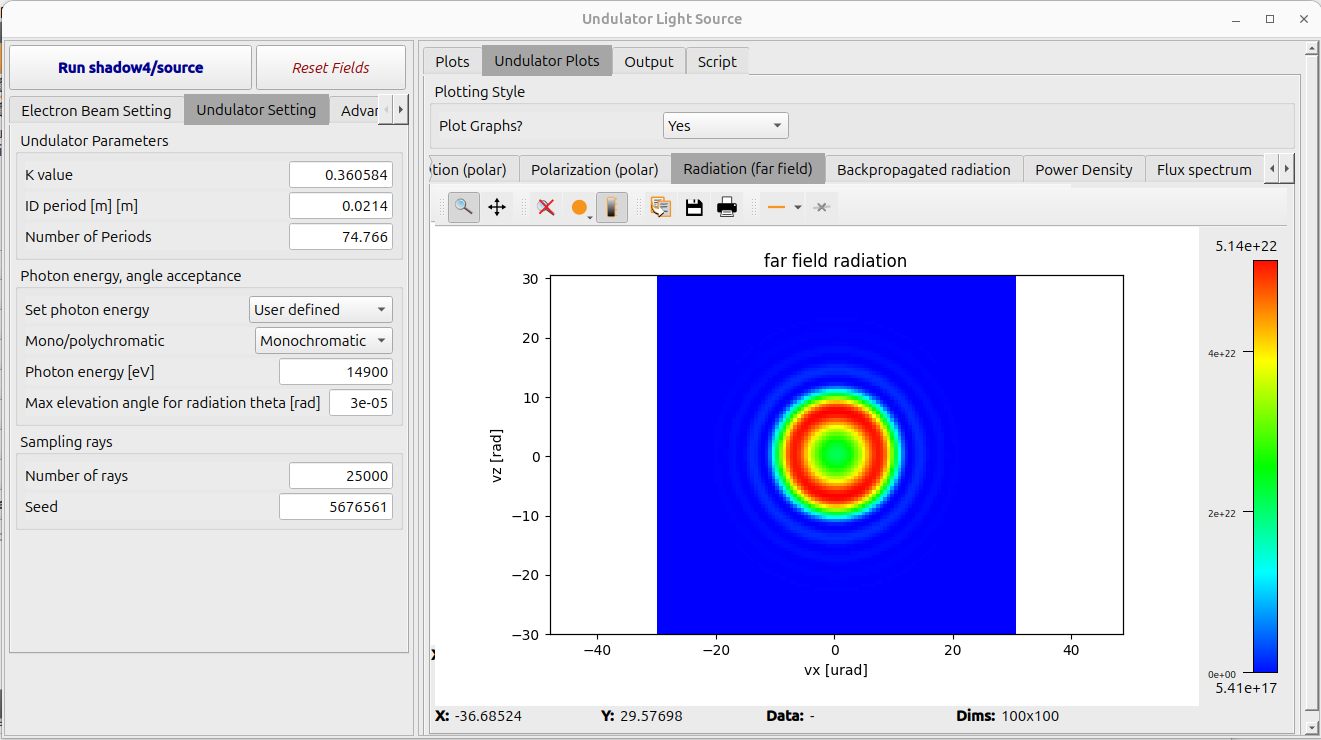
\includegraphics[width=0.7\textwidth]{undulators/fig3c.png}
\end{figure}

If you want, you can calculate the real size by backpropagating the far field radiation. figure~\ref{fig:id-fig4} shows an example of how to set the parameters to get ``resonable" results. 

\begin{figure}[H]
\label{fig:id-fig4}
\caption{In the ``Undulator Light Source" widget, manual set of the backpropagating the far field radiation at resonance $E_1$ (top), at $E_1+$100 eV (center), and $E_1-$100 eV (bottom).}
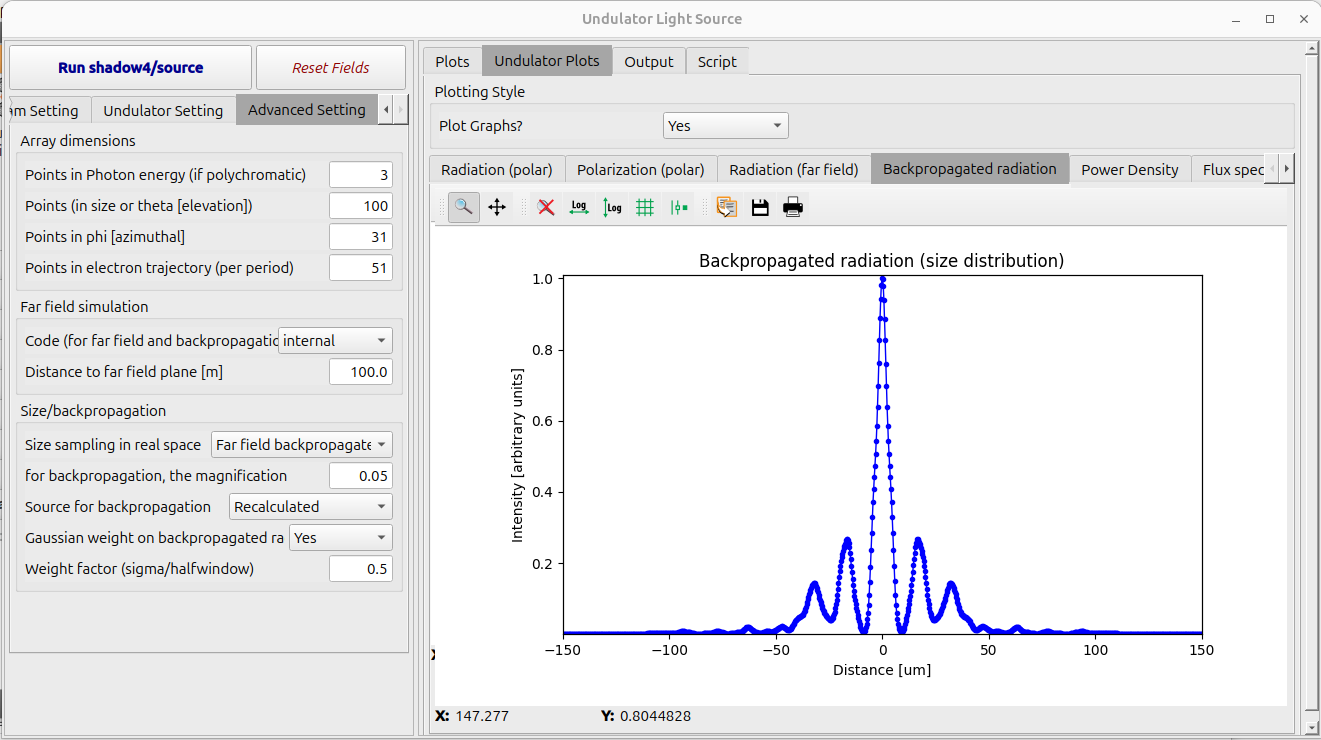
\includegraphics[width=0.7\textwidth]{undulators/fig4.png}
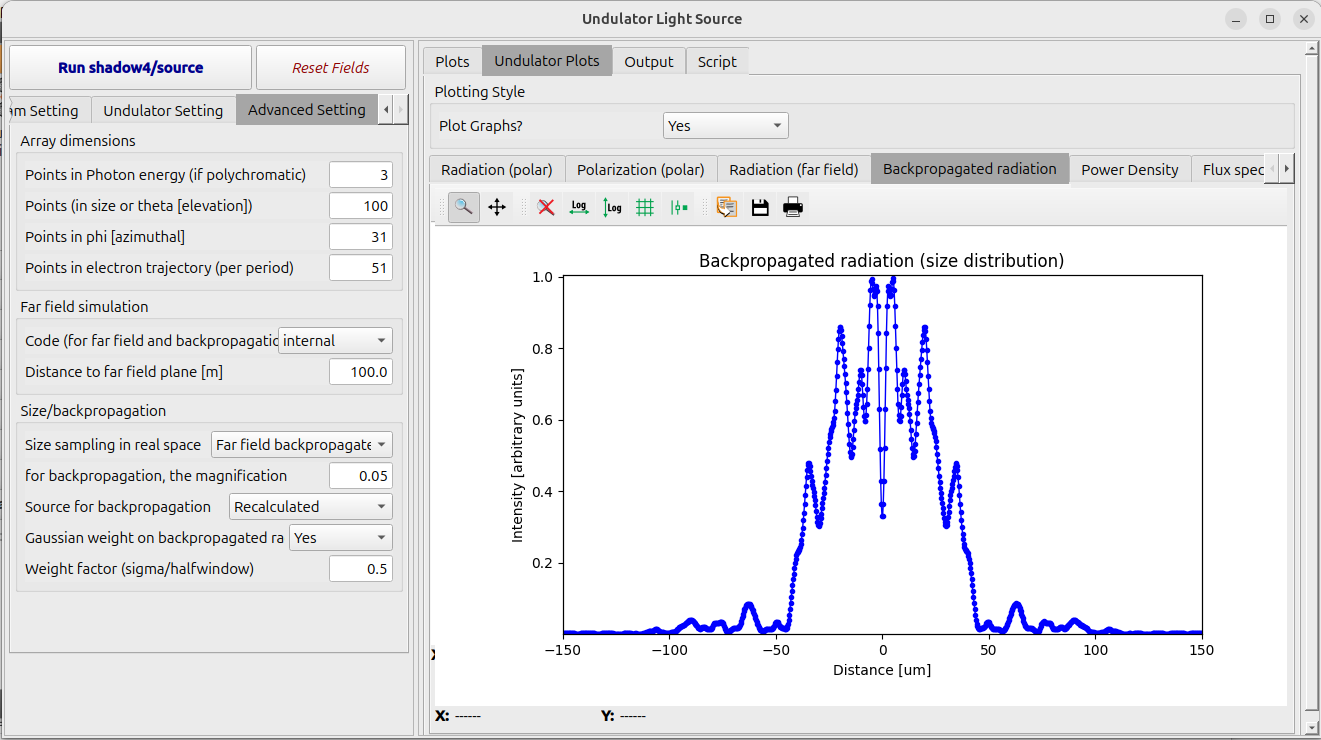
\includegraphics[width=0.7\textwidth]{undulators/fig4b.png}
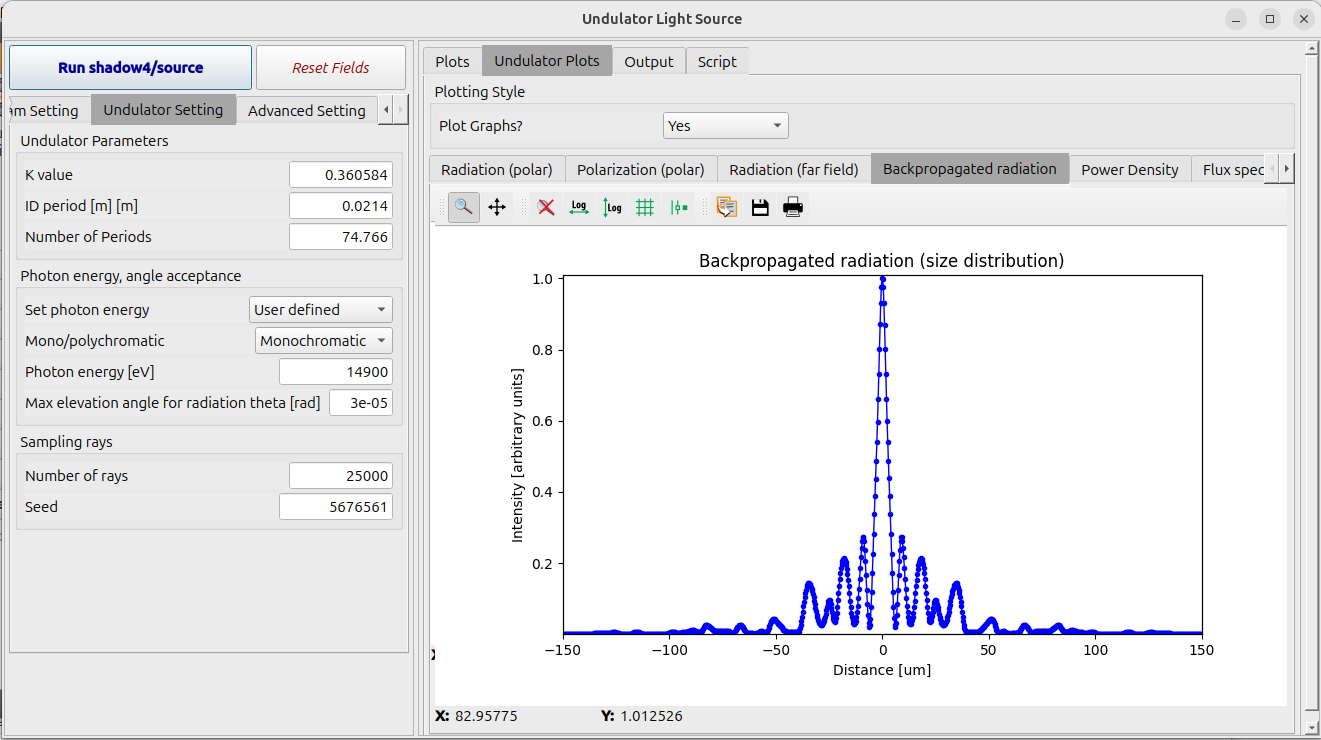
\includegraphics[width=0.7\textwidth]{undulators/fig4c.png}
\end{figure}

A comparison of the sizes and divergences obtained is in Table~\ref{tab:full}

\begin{table}[H]
\centering
\caption{Sizes and divergences from several ``Undulator Light Source" runs.}
\begin{tabular}{lccc}
\hline
\textbf{Energy} & \textbf{Value} & \textbf{Size} $\mu$m& \textbf{Divergence} $\mu$rad\\
\hline
Monochromatic & 15000 & 87.7 $\times$ 41.3& 13.2 $\times$ 13.3 \\
Monochromatic & 15100 & 85.9 $\times$ 41.6& 13.6 $\times$ 7.3 \\
Monochromatic & 14900 & 92.0 $\times$ 41.7& 17.8 $\times$ 16.8 \\
\hline
Polychromatic & 14900-15100 & 93.5 $\times$ 46.3& \textcolor{red}{30.5 $\times$ 36.6} \\

\hline
\end{tabular}
\label{tab:full}
\end{table}

iv) Set the polychromatic option, and in ``Advanced Setting" input the wanted number of energy point (the calculation becomes slow!).
Results are in Table~\ref{tab:full}.


